% Figure 4 — The Soma-Field Instrument Pipeline
% Compile: lualatex fig4_instrument.tex
% Produces fig4_instrument.pdf
%
% Biofeedback → Soma-Field model → Emotion vector → Tensor/score → Synthesis

\documentclass[tikz, border=4pt]{standalone}
\usepackage{tikz}
\usetikzlibrary{arrows.meta, positioning, shapes.geometric, shapes.multipart}

\begin{document}
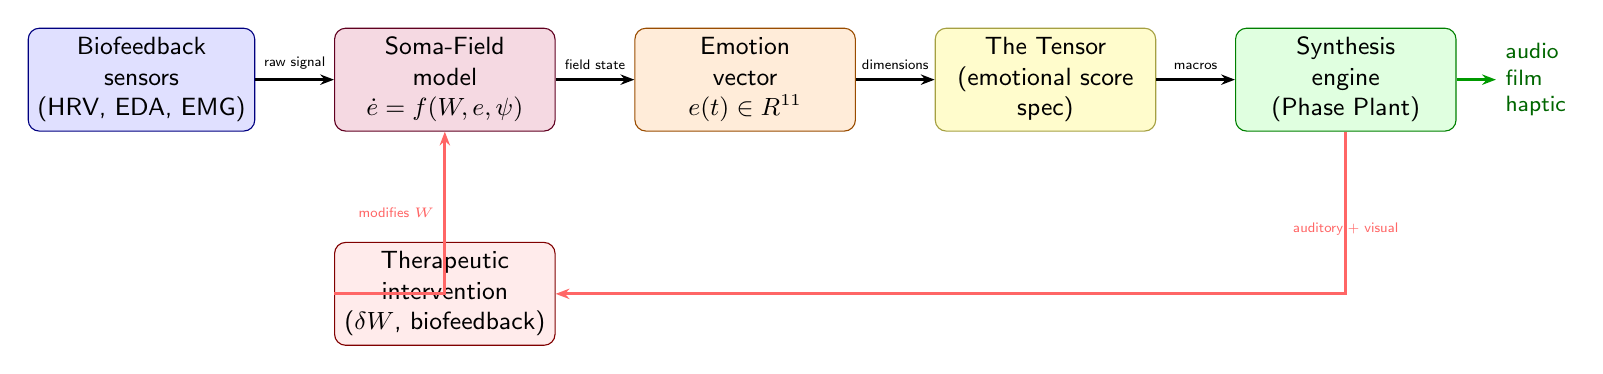
\begin{tikzpicture}[
  block/.style  = {rectangle, rounded corners=4pt, minimum width=2.8cm,
                   minimum height=1.0cm, align=center,
                   font=\sffamily\small, draw},
  arrow/.style  = {-{Stealth[length=5pt]}, line width=1.0pt},
  node distance = 0.8cm and 1.0cm,
  every node/.append style={font=\sffamily\small}
]

% ── Signal chain (left → right) ──────────────────────────────────────────────
\node[block, fill=blue!12, draw=blue!50!black]
  (bio) {Biofeedback\\sensors\\(HRV, EDA, EMG)};

\node[block, fill=purple!15, draw=purple!50!black, right=of bio]
  (sf)  {Soma-Field\\model\\$\dot{e} = f(W,e,\psi)$};

\node[block, fill=orange!15, draw=orange!60!black, right=of sf]
  (ev)  {Emotion\\vector\\$e(t) \in \mathbb{R}^{11}$};

\node[block, fill=yellow!20, draw=yellow!60!black, right=of ev]
  (tens) {The Tensor\\(emotional score\\spec)};

\node[block, fill=green!12, draw=green!50!black, right=of tens]
  (synth) {Synthesis\\engine\\(Phase Plant)};

% ── Arrows ───────────────────────────────────────────────────────────────────
\draw[arrow] (bio)  -- (sf)    node[midway,above,font=\sffamily\tiny] {raw signal};
\draw[arrow] (sf)   -- (ev)    node[midway,above,font=\sffamily\tiny] {field state};
\draw[arrow] (ev)   -- (tens)  node[midway,above,font=\sffamily\tiny] {dimensions};
\draw[arrow] (tens) -- (synth) node[midway,above,font=\sffamily\tiny] {macros};

% ── Feedback loop (therapeutic W modification) ────────────────────────────────
\node[block, fill=red!8, draw=red!50!black, below=1.4cm of sf]
  (ther) {Therapeutic\\intervention\\($\delta W$, biofeedback)};

\draw[arrow, red!60] (synth.south) |- (ther.east)
  node[near start, below, font=\sffamily\tiny] {auditory + visual};
\draw[arrow, red!60] (ther.west)  -| (sf.south)
  node[near end, left, font=\sffamily\tiny] {modifies $W$};

% ── Output annotation ─────────────────────────────────────────────────────────
\node[right=0.5cm of synth, align=left, font=\sffamily\footnotesize, text=green!40!black]
  (out) {audio\\film\\haptic};
\draw[arrow, green!60!black] (synth.east) -- (out.west);

\end{tikzpicture}
\end{document}
